\documentclass[10pt,a4paper]{beamer}
\usetheme{Malmoe}
\definecolor{UniGreen}{RGB}{0,100,200}
\setbeamercolor{title}{fg=UniGreen}
\setbeamercolor{frametitle}{fg=UniGreen}
\setbeamercolor{structure}{fg=UniGreen}
\usepackage[utf8]{inputenc}
\usepackage[MeX]{polski}
\usepackage{amsmath}
\usepackage{amsfonts}
\usepackage{amssymb}
\usepackage{graphicx}
\usepackage{rotating}
\usepackage{multirow}
\usepackage{array}
\usepackage{tikz}
\usetikzlibrary{shapes,arrows}
\usepackage{pgfplots}
\pgfplotsset{compat=1.8}
\author{\texorpdfstring{Jakub Turek \newline \href{mailto:jkbturek@gmail.com}{ jkbturek@gmail.com }}{Jakub Turek}}
\title{Wykorzystanie sztucznej inteligencji w grze Scrabble}
\institute{Wydział Elektroniki i Technik Informacyjnych}
\begin{document}

\begin{frame}
	\titlepage
\end{frame}

\section{Wstęp}

\begin{frame}
	\begin{block}{Scrabble}
		\textbf{Gra słowna polegająca na układaniu na określonej planszy wyrazów z~losowanych liter.}
		
		\vspace{10mm}
		
		\emph{Wielki słownik ortograficzny - PWN 2003, 2006, 2008 - E. Polański}
	\end{block}
\end{frame}

\begin{frame}
	\frametitle{Historia Scrabble}
	
	\begin{itemize}
		\item 1938 r. - gra \emph{Lexiko}, Alfred Mosher Butts.
		\item Lata 40. - \emph{Criss-Crossword} - udoskonalona wersja \emph{Lexiko}.
		\item 1948 r. - James Burnot, \emph{Scrabble}.
		\item Lata 80. - Hasbro.
		\item Lata 80. - teleturniej \emph{Scrabble}.
		\item Obecnie - 121 krajów, 29 różnych języków.
		\item Do chwili obecnej - 150 milionów sprzedanych egzemplarzy.
	\end{itemize}
\end{frame}

\subsection{Zasady}

\begin{frame}
	\frametitle{Plansza}
	
	\begin{columns}[onlytextwidth]
		\begin{column}{0.55\textwidth}
			\includegraphics[scale=0.17]{graphics/board.jpg}
		\end{column}
		\begin{column}{0.45\textwidth}
			\begin{itemize}
				\item Wymiary $15 \times 15$.
				\item Premie:
					\begin{itemize}
						\item literowe:
							\begin{itemize}
								\item podwójna,
								\item potrójna.
							\end{itemize}
						\item słowne:
							\begin{itemize}
								\item podwójna,
								\item potrójna.
							\end{itemize}
					\end{itemize}
				\item Środek planszy:
					\begin{itemize}
						\item pierwszy wyraz musi przechodzić przez pole,
						\item podwójna premia słowna.
					\end{itemize}
			\end{itemize}
		\end{column}
	\end{columns}
\end{frame}

\begin{frame}
	\frametitle{Płytki (polska wersja)}
	
	\begin{columns}[onlytextwidth]
		\begin{column}{0.55\textwidth}
			\scalebox{0.8}{
				\begin{tabular}{|c|c|c||c|c|c||c|c|c|}
					\hline
					\multirow{16}{*}{
						\begin{sideways}
							Litera
						\end{sideways}	} &
					\multirow{16}{*}{
						\begin{sideways}
							Ilość płytek
						\end{sideways}} & 
					\multirow{16}{*}{
						\begin{sideways}
							Liczba punktów
						\end{sideways}} & \textbf{A} & 9 & 1 & \textbf{M} & 3 & 2 \\
					\cline{4-9}
					&&& \textbf{Ą} & 1 & 5 & \textbf{N} & 5 & 1 \\
					\cline{4-9}
					&&& \textbf{B} & 2 & 3 & \textbf{Ń} & 1 & 7 \\			
					\cline{4-9}
					&&& \textbf{C} & 3 & 2 & \textbf{O} & 6 & 1 \\			
					\cline{4-9}
					&&& \textbf{Ć} & 1 & 6 & \textbf{Ó} & 1 & 5 \\
					\cline{4-9}
					&&& \textbf{D} & 3 & 2 & \textbf{P} & 3 & 2 \\	
					\cline{4-9}
					&&& \textbf{E} & 7 & 1 & \textbf{R} & 4 & 1 \\
					\cline{4-9}
					&&& \textbf{Ę} & 1 & 5 & \textbf{S} & 4 & 1 \\
					\cline{4-9}
					&&& \textbf{F} & 1 & 5 & \textbf{Ś} & 1 & 5 \\
					\cline{4-9}				
					&&& \textbf{G} & 2 & 3 & \textbf{T} & 3 & 2 \\
					\cline{4-9}
					&&& \textbf{H} & 2 & 3 & \textbf{U} & 2 & 3 \\
					\cline{4-9}
					&&& \textbf{I} & 8 & 1 & \textbf{W} & 4 & 1 \\
					\cline{4-9}
					&&& \textbf{J} & 2 & 3 & \textbf{Y} & 4 & 2 \\
					\cline{4-9}
					&&& \textbf{K} & 3 & 2 & \textbf{Z} & 5 & 1 \\
					\cline{4-9}
					&&& \textbf{L} & 3 & 2 & \textbf{Ź} & 1 & 9 \\
					\cline{4-9}
					&&& \textbf{Ł} & 2 & 3 & \textbf{Ż} & 1 & 5 \\
					\hline
				\end{tabular}
			}
		\end{column}
		\begin{column}{0.45\textwidth}
			\begin{itemize}
				\item 98 płytek z~literami.
				\item Każda litera ma przyporządkowaną punktację.
				\item Ilość płytek proporcjonalna do częstotliwości występowania litery.
				\item Punktacja odwrotnie proporcjonalna do częstotliwości występowania litery.
				\item 2 \emph{blanki}.
			\end{itemize}
		\end{column}
	\end{columns}
\end{frame}

\begin{frame}
	\frametitle{Reguły}
	
	\begin{itemize}
		\item Na stojaku 7 wylosowanych płytek.
		\item Naprzemienne ruchy.
		\item Prawidłowy ruch:
			\begin{itemize}
				\item Płytki wyłożone w~jednym wierszu (lub kolumnie) w~sposób ciągły.
				\item Wykorzystanie przynajmniej jednej litery znajdującej się już na planszy.
				\item Tworzy poprawny wyraz czytany od lewej do prawej (lub od góry do dołu).
				\item Wszystkie płytki przylegające tworzą poprawne wyrazy w~układzie krzyżówkowym.
			\end{itemize}
		\item Koniec gry - pierwszy gracz, który nie ma płytek na stojaku.
		\item Wygrywa gracz z~największą liczbą punktów.
	\end{itemize}
\end{frame}

\begin{frame}
	\frametitle{Dopuszczalne słowa}
	
	Dopuszczalne jest wykorzystanie wszystkich słów znajdujących się w~dowolnym słowniku języka polskiego (wraz z~poprawnymi odmianami) z~wyłączeniem:
	
	\begin{itemize}
		\item nazw własnych (wyrazów pisanych z~wielkiej litery),
		\item skrótów,
		\item przedrostków, przyrostków,
		\item wyrazów wymagających użycia apostrofu lub łącznika.
	\end{itemize}
\end{frame}

\section{Słowniki}
\subsection{Polskie słowniki wyrazów do gier}

\begin{frame}[fragile]
	\frametitle{Słownik wyrazów do gier}
	
	\textbf{Słownik wyrazów do gier} to lista wszystkich słów, wraz ze wszystkimi poprawnymi odmianami, dopuszczalnych do wykorzystania w~grach słownych. 
	
	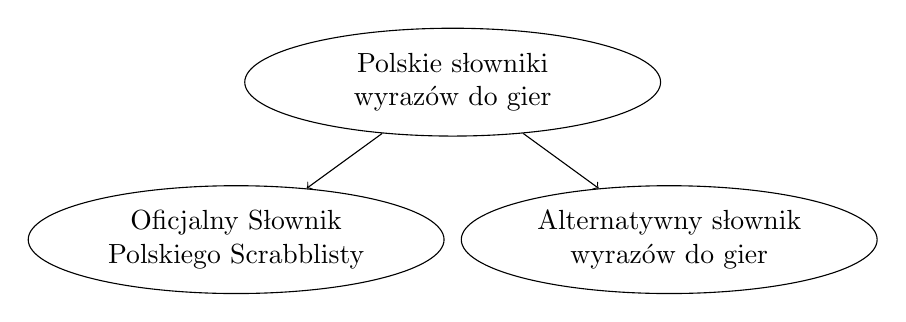
\begin{tikzpicture}
		\tikzstyle{every node}=[draw, shape=ellipse, text width=3.5cm, align=center];
		\node (alternative) at (2.75, -2) {Alternatywny słownik wyrazów do gier};
        \node (pfs) at (-2.75, -2) {Oficjalny Słownik Polskiego Scrabblisty};
		\node (dictionaries) at (0, 0) {Polskie słowniki wyrazów do gier};
		\draw[->] (dictionaries) -- (pfs);
		\draw[->] (dictionaries) -- (alternative);
	\end{tikzpicture}
\end{frame}

\begin{frame}
	\frametitle{Porównanie OSPS i~słownika alternatywnego}
	
	\scalebox{0.75}{
		\begin{tabular}{|l|c|c|}
			\cline{2-3}
			\multicolumn{1}{c|}{} & \textbf{OSPS} & \textbf{Słownik alternatywny} \\
			\hline
			\multirow{2}{*}{Wydawca} & Polska Federacja Scrabble, & \multirow{2}{*}{Serwis z~grami online Kurnik} \\
			& Polskie Wydawnictwo Naukowe & \\
			\hline
			Przeznaczenie & Gry turniejowe & Gra ,,Literaki'' \\
			\hline
			Liczba słów & 2 477 212 & 2 703 830 \\
			\hline
			\multirow{3}{*}{Źródło} & Zamknięta lista słowników języka & Otwarta lista słowników języka \\
			& polskiego, ortograficznych, wyrazów & polskiego, ortograficznych, \\
			& obcych wydawnictwa PWN & wyrazów obcych \\
			\hline
			\multirow{6}{*}{Przykładowe różnice} & \multicolumn{1}{l|}{\textcolor{UniGreen}{$\blacktriangleright$} basfu}  & \multicolumn{1}{l|}{\textcolor{UniGreen}{$\blacktriangleright$} aeolipile} \\
			& \multicolumn{1}{l|}{\textcolor{UniGreen}{$\blacktriangleright$} gral} & \multicolumn{1}{l|}{\textcolor{UniGreen}{$\blacktriangleright$} donowi} \\
			& \multicolumn{1}{l|}{\textcolor{UniGreen}{$\blacktriangleright$} meru} & \multicolumn{1}{l|}{\textcolor{UniGreen}{$\blacktriangleright$} feroce} \\
			& \multicolumn{1}{l|}{\textcolor{UniGreen}{$\blacktriangleright$} noblów} & \multicolumn{1}{l|}{\textcolor{UniGreen}{$\blacktriangleright$} geez} \\
			& \multicolumn{1}{l|}{\textcolor{UniGreen}{$\blacktriangleright$} późńmyż} & \multicolumn{1}{l|}{\textcolor{UniGreen}{$\blacktriangleright$} tyiyn} \\
			& \multicolumn{1}{l|}{\textcolor{UniGreen}{$\blacktriangleright$} szwed} & \multicolumn{1}{l|}{\textcolor{UniGreen}{$\blacktriangleright$} żad} \\
			\hline
		\end{tabular}
	}
\end{frame}

\begin{frame}

	\begin{center}
		\LARGE{Dalsze rozważania przeprowadzane będą dla słownika alternatywnego.}
	\end{center}

\end{frame}

\subsection{Statystyka}

\begin{frame}
	\frametitle{Statystyczny opis słownika}
	
	Na podstawie statystycznego opisu słownika można wyprowadzić szereg użytecznych heurystyk:
	
	\begin{itemize}
		\item Częstotliwość występowania liter.
		\item Najbardziej prawdopodobne n-gramy.
		\item Najlepsze otwarcia.
		\item Najlepsze kombinacje liter.
	\end{itemize}
\end{frame}

\begin{frame}[fragile]
	\frametitle{Prawdopodobieństwo występowania liter}
			
		\begin{tikzpicture}
			\begin{axis}[	ytick={0, 0.01, ..., 0.1}, 
					yticklabel style={/pgf/number format/fixed},
					bar width=2mm,
					symbolic x coords={a,i,o,e,n,y,z,w,r,c,m,s,k,p,t,u,l,d,el,j,b,g,on,h,es,zet,een,f,uu,en,ci,ziet},
					xticklabels={a,i,o,e,n,y,z,w,r,c,m,s,k,p,t,u,l,d,ł,j,b,g,ą,h,ś,ż,ę,f,ó,ń,ć,ź},
					xticklabel style={text height=1.5ex},
					xtick=data,
					legend entries={Prawdopodobieństwo dla słownika,Prawdopodobieństwo w Scrabble},
					height=.9\textheight,
					width=\textwidth	]
					
    			\addplot[ybar,fill=UniGreen, area legend] coordinates {
        			(a,0.0937997771175)
        			(i,0.0894002903657)
        			(o,0.0796720098207)
        			(e,0.0765123987403)
        			(n,0.0683027202572)
        			(y,0.0497071483395)
        			(z,0.0466694841626)
        			(w,0.0453746978807)
        			(r,0.0440417929225)
        			(c,0.0409715964269)
        			(m,0.0387468458849)
        			(s,0.0322800452968)
        			(k,0.0316402758911)
        			(p,0.029784849318)
        			(t,0.0273647734205)
        			(u,0.0271062565005)
        			(l,0.023888810187)
        			(d,0.0219487338635)
        			(el,0.0210803509823)
        			(j,0.0195483416618)
        			(b,0.0192369186479)
        			(g,0.0132131819509)
        			(on,0.0128586125387)
        			(h,0.0115084555932)
        			(es,0.0096922978289)
        			(zet,0.0064777761380)
        			(een,0.0064627258330)
        			(f,0.0044409243818)
        			(uu,0.0035346199898)
        			(en,0.0027972207673)
        			(ci, 0.0011952505312)
        			(ziet,0.0007161382021)
    			};
    			
    			\addplot[ybar,fill=lightgray, area legend] coordinates {
        			(a,0.09)
        			(i,0.08)
        			(o,0.06)
        			(e,0.07)
        			(n,0.05)
        			(y,0.04)
        			(z,0.05)
        			(w,0.04)
        			(r,0.04)
        			(c,0.03)
        			(m,0.03)
        			(s,0.04)
        			(k,0.03)
        			(p,0.03)
        			(t,0.03)
        			(u,0.02)
        			(l,0.03)
        			(d,0.03)
        			(el,0.02)
        			(j,0.02)
        			(b,0.02)
        			(g,0.02)
        			(on,0.01)
        			(h,0.02)
        			(es,0.01)
        			(zet,0.01)
        			(een,0.01)
        			(f,0.01)
        			(uu,0.01)
        			(en,0.01)
        			(ci, 0.01)
        			(ziet,0.01)
    			};
    			\addplot[forget plot,ybar,fill=UniGreen] coordinates {
        			(a,0)
        			(i,0)
        			(o,0)
        			(e,0)
        			(n,0)
        			(y,0)
        			(z,0.0466694841626)
        			(w,0)
        			(r,0)
        			(c,0)
        			(m,0)
        			(s,0.0322800452968)
        			(k,0)
        			(p,0.029784849318)
        			(t,0.0273647734205)
        			(u,0)
        			(l,0.023888810187)
        			(d,0.0219487338635)
        			(el,0)
        			(j,0.0195483416618)
        			(b,0.0192369186479)
        			(g,0.0132131819509)
        			(on,0)
        			(h,0.0115084555932)
        			(es,0.0096922978289)
        			(zet,0.0064777761380)
        			(een,0.0064627258330)
        			(f,0.0044409243818)
        			(uu,0.0035346199898)
        			(en,0.0027972207673)
        			(ci, 0.0011952505312)
        			(ziet,0.0007161382021)
    			};
			\end{axis}
		\end{tikzpicture}
\end{frame}

\begin{frame}
	\frametitle{Prawdopodobieństwo występowania bigramów}
	
	\begin{columns}
		\begin{column}{.5\textwidth}
			\begin{block}{N-gram}
				Sekwencja składająca się z n~liter, znaków lub wyrazów.
			\end{block}
			
		\begin{itemize}
			\item Unigram.
			\item Bigram.
			\item Trigram.
			\item 4-gram.
			\item ...
			\item N-gram.
		\end{itemize}
		
		\end{column}
		
		\begin{column}{.5\textwidth}
			\begin{tabular}{|c|c|}
				\hline
				Bigram	&	Wystąpienia	\\
				\hline
				ni		&	1 077 436	\\
				ie		&	1 028 249	\\
				ow	&	645 018		\\
				an		&	507 205		\\
				wa	&	484 295		\\
				za		&	313 370		\\
				po		&	301 636		\\
				ch		&	296 749		\\
				ał		&	294 734		\\
				ia		&	284 247		\\
				\hline
			\end{tabular}

		\end{column}

	\end{columns}

\end{frame}

\begin{frame}
	\frametitle{Prawdopodobieństwo występowania n-gramów}
	
	\begin{columns}
		\begin{column}{.3\textwidth}
			\scalebox{.8}{
				\begin{tabular}{|c|c|}
					\hline
					Trigram	&	Wystąpienia	\\
					\hline
					nie	&	635 196	\\
					owa	&	307 277	\\
					ani	&	195 186	\\
					wan	&	180 460	\\
					cie	&	148 513	\\
					nia	&	142 201	\\
					jąc	&	131 792	\\
					prz	&	130 283	\\
					wał	&	126 134	\\
					rze	&	116 370	\\
					\hline
				\end{tabular}
			}

		\end{column}
		
		\begin{column}{.3\textwidth}
			\scalebox{.8}{
				\begin{tabular}{|c|c|}
					\hline
					4-gram	&	Wystąpienia	\\
					\hline
					owan	&	127 626	\\
					ował		&	88 130		\\
					wani		&	78 095		\\
					niep		&	77 449		\\
					prze		&	73 230		\\
					ując		&	67 062		\\
					ania		&	61 398		\\
					ając		&	59 499		\\
					ście		&	56 462		\\
					łaby		&	55 380		\\
					\hline
				\end{tabular}
			}

		\end{column}
		
		\begin{column}{.3\textwidth}
			\scalebox{.8}{
				\begin{tabular}{|c|c|}
					\hline
					5-gram	&	Wystąpienia	\\
					\hline
					owani	&	54 991	\\
					niepo	&	40 329	\\
					ałaby	&	37 581	\\
					yście		&	33 161	\\
					owała	&	28 175	\\
					niewy	&	26 193	\\
					owane	&	25 555	\\
					wania	&	25 551	\\
					owany	&	25 542	\\
					ałyby	&	25 282	\\
					\hline
				\end{tabular}
			}

		\end{column}

	\end{columns}
\end{frame}

\begin{frame}
	\frametitle{Prawdopodobieństwo występowania n-gramów (2)}
	
	\begin{columns}
		\begin{column}{.5\textwidth}
				\begin{tabular}{|c|c|}
					\hline
					6-gram	&	Wystąpienia	\\
					\hline
					owania	&	17 609	\\
					wałaby	&	17 161	\\
					byście	&	16 821	\\
					liście		&	15 910	\\
					aniami	&	15 585	\\
					aniach	&	15 585	\\
					łyście	&	15 405	\\
					owanie	&	14 674	\\
					owałby	&	14 437	\\
					nieprz	&	14 328	\\
					\hline
				\end{tabular}
		\end{column}
		
		\begin{column}{.5\textwidth}
				\begin{tabular}{|c|c|}
					\hline
					7-gram	&	Wystąpienia	\\
					\hline
					owałaby	&	12 401		\\
					libyśmy		&	12 267		\\
					łybyśmy	&	12 094		\\
					ałyście		&	9 902		\\
					aliście		&	9 304		\\
					ibyście		&	8 445		\\
					libyści		&	8 443		\\
					ybyście		&	8 317		\\
					łybyści		&	8 314		\\
					nieprze		&	8 111		\\
					\hline
				\end{tabular}
		\end{column}
	\end{columns}
\end{frame}

\end{document}